All SimCenter applications are available at
the \href{https://simcenter.designsafe-ci.org/research-tools/overview/}{SimCenter
website} under \emph{Research Tools}. The following sections outline
the steps necessary to download and install the \texttt{\getsoftwarename{}}
application. The SimCenter applications do require that you install a
number of other applications that are needed to run the workflows on
your local machine as well as at DesignSafe. \\


%===============================================================================
\section{Download the Application}
%===============================================================================

% \subsection{Download the Application Files}

To download the \texttt{\getsoftwarename{}} application navigate to
the \getsoftwarepage{\texttt{\getsoftwarename{}} page} and click on
the \emph{Download App \& User Manual} link on the right side of the
page. As shown in \Cref{fig:app_choose_file}, this will bring you to another page which contains a list of downloadable files and directories.

\softwareSwitch{PBE}{
\begin{figure}[!htbp]
  \centering {
    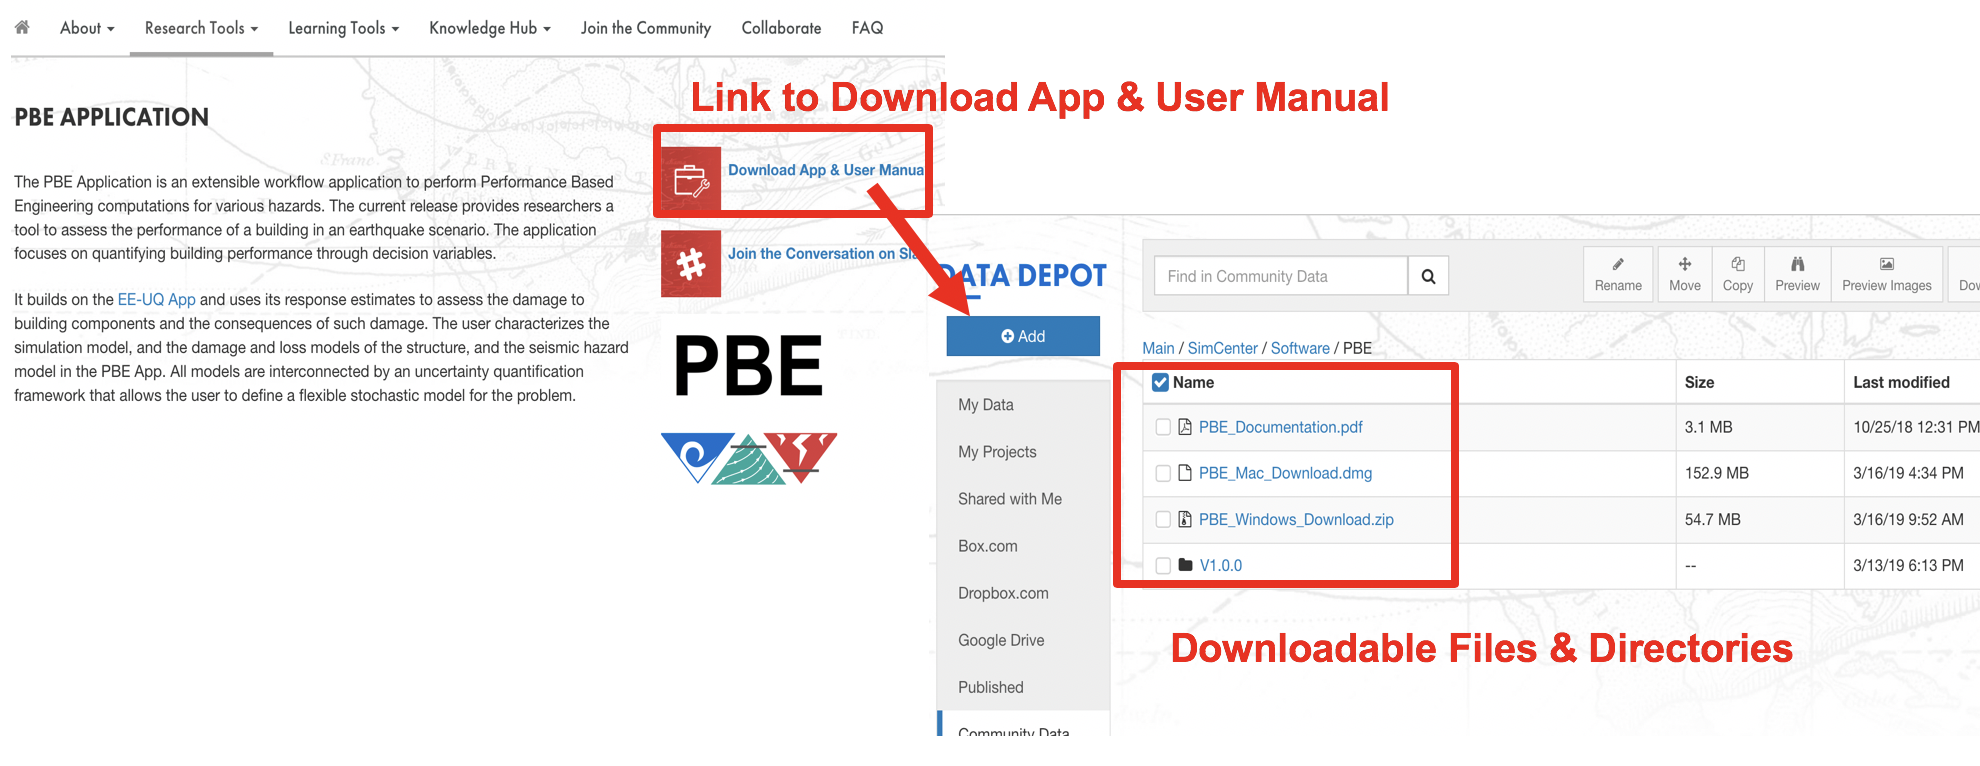
\includegraphics[width=0.95\textwidth]
    {installation/figures/pbeDownload.png} }
  \caption{Download Application}
  \label{fig:app_choose_file}
\end{figure}
}{}

\softwareSwitch{EE-UQ}{
\begin{figure}[!htbp]
  \centering {
    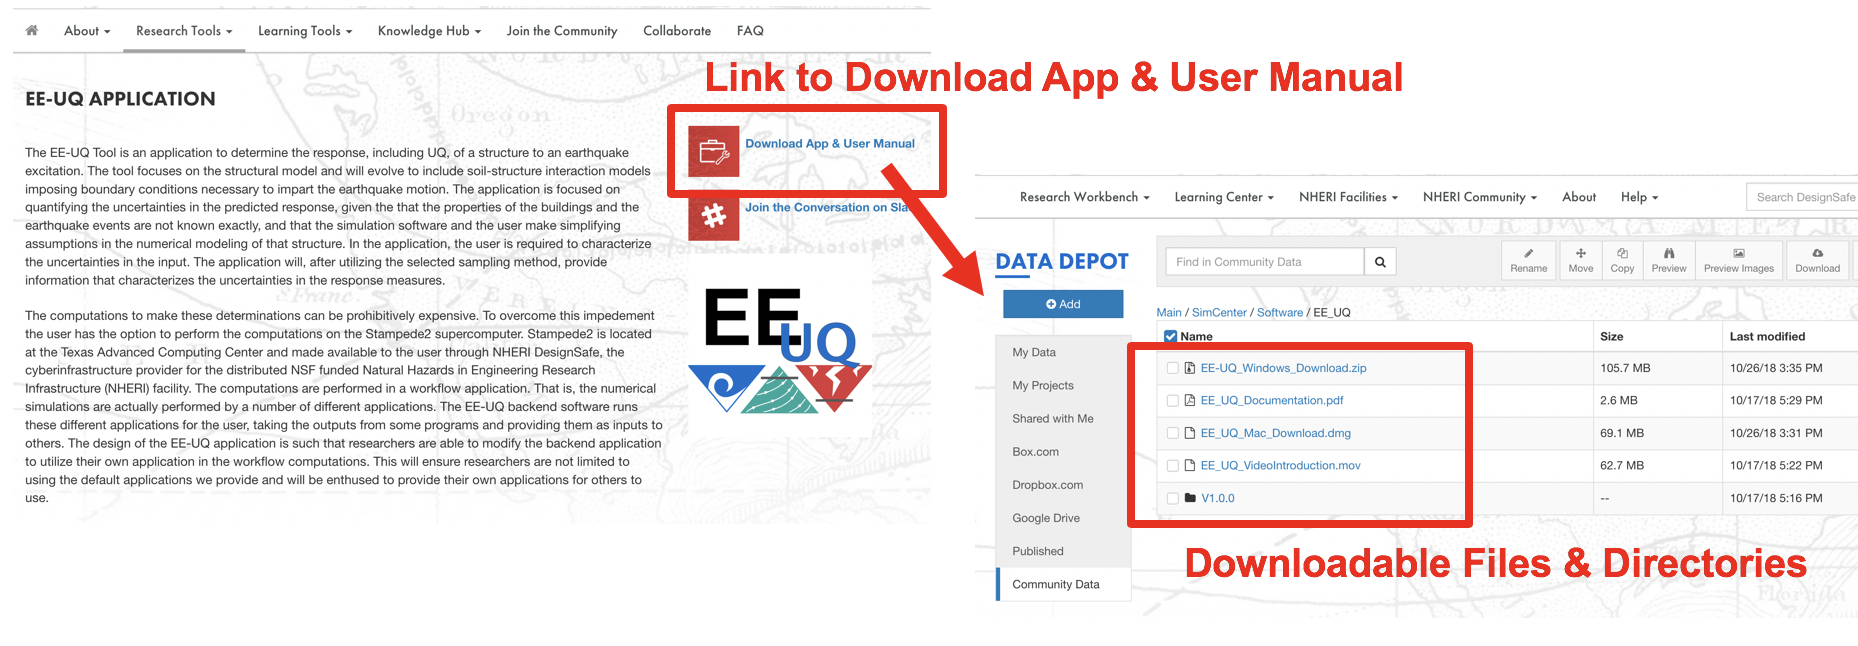
\includegraphics[width=0.95\textwidth]
    {installation/figures/eeDownload.png} }
  \caption{Download Application}
  \label{fig:app_choose_file}
\end{figure}
}{}

\softwareSwitch{WE-UQ}{
\begin{figure}[!htbp]
  \centering {
    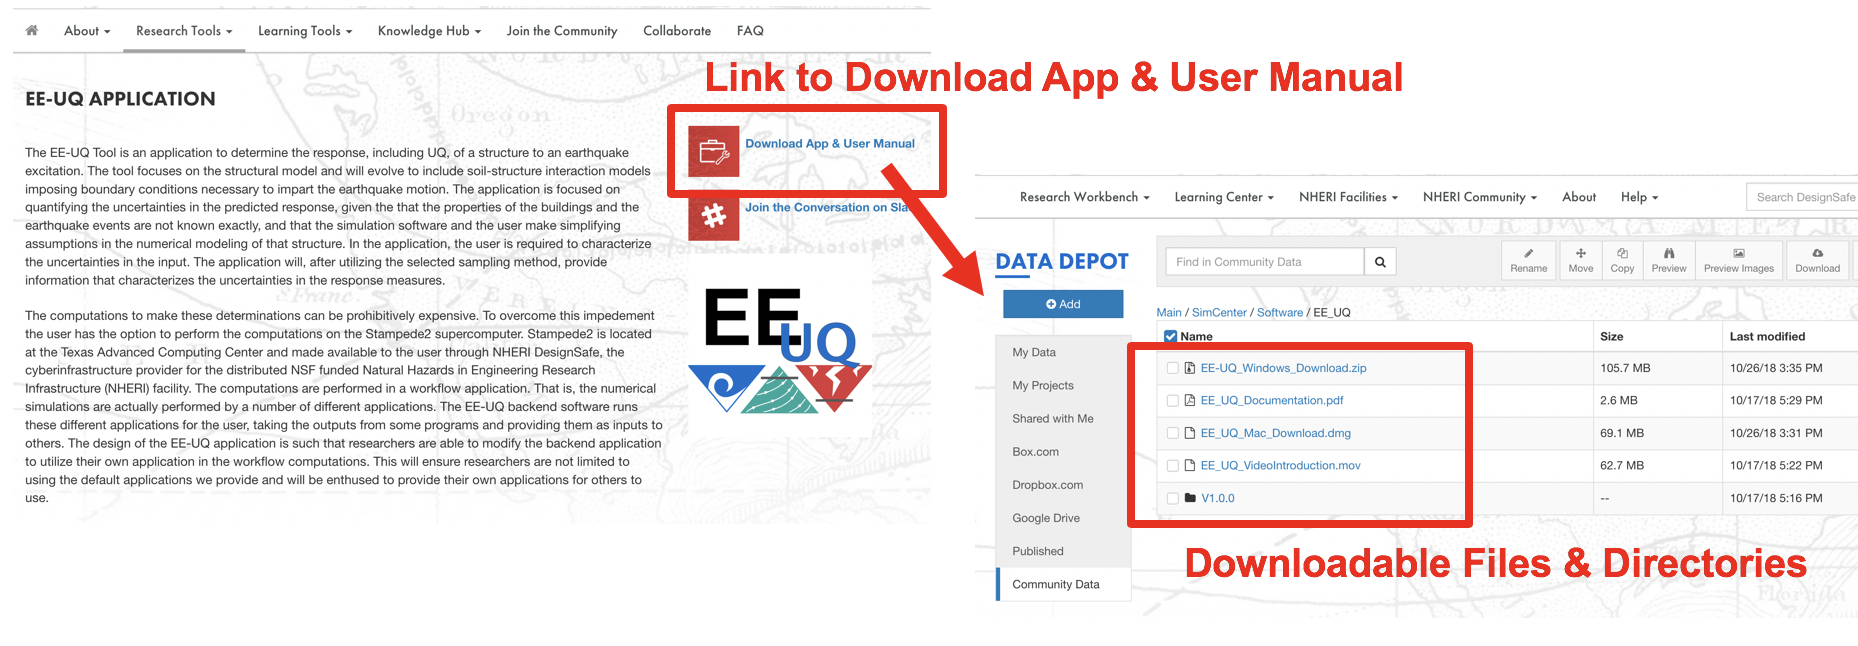
\includegraphics[width=0.95\textwidth]
    {installation/figures/eeDownload.png} }
  \caption{Download Application}
  \label{fig:app_choose_file}
\end{figure}
}{}


There are at least four files available for download from this page: 
\begin{enumerate}
    \item The PDF file is the User Manual that you are reading now.
    \item The MOV file is an video that provides an introduction to the usage of the application.
    \item The ZIP file is an archive that contains the application files for a Windows operating system.
    \item The DMG file is an archive that contains the application files for a Mac OS X operating system.
\end{enumerate}

To download the \texttt{\getsoftwarename{}} application click on the link for
the appropriate file for your operating system and then click on the
Download button at bottom right corner of the ensuing pop-up window. 
Unpackage the application from the downloaded
file and place it in a location on your filesystem. On Windows, we
recommend that you create a \texttt{C:/SimCenter/\getsoftwarename{}}
directory and extract the contents of the \texttt{ZIP} archive
there. It is also recommended to run the included installer for Visual C/C++ runtime library(vc\_redist.x64.exe). 
If you use a Mac we recommend you copy the application to either your
home folder or your Desktop folder. You are free to place the
applications anywhere you wish, you will need to make the
appropriate adjustments with the following instructions if you do so. \\

Now test that the application starts. To do this navigate to
the location where you placed the application and open it. You should
see the user interface (UI) shown in \Cref{fig:app_UI} after
starting the application. Now Quit the application. Additional steps are required before 
computations can be performed.\\

\softwareSwitch{PBE}{
\begin{figure}[!htbp]
  \centering {
    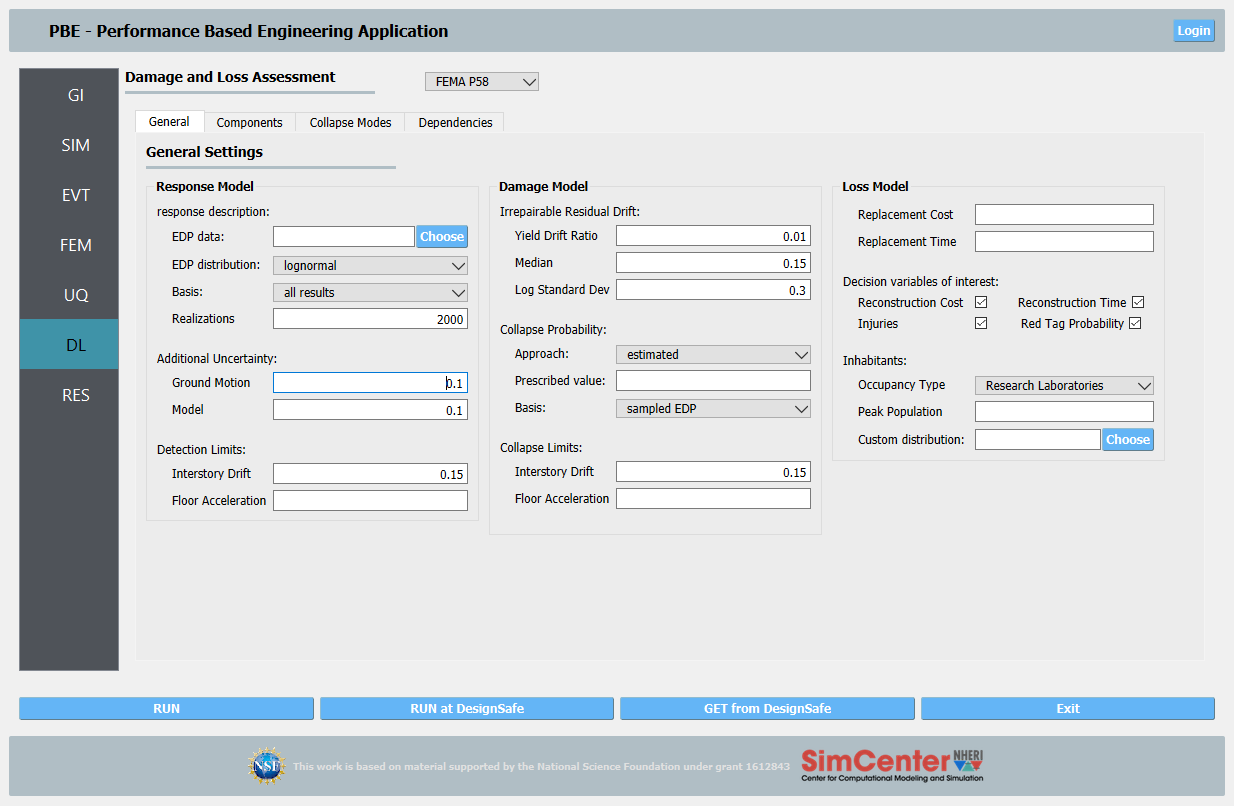
\includegraphics[width=0.95\textwidth]
    {installation/figures/PBE.png} }
  \caption{PBE Application on Startup}
  \label{fig:app_UI}
\end{figure}
}{}

\softwareSwitch{EE-UQ}{
\begin{figure}[!htbp]
  \centering {
    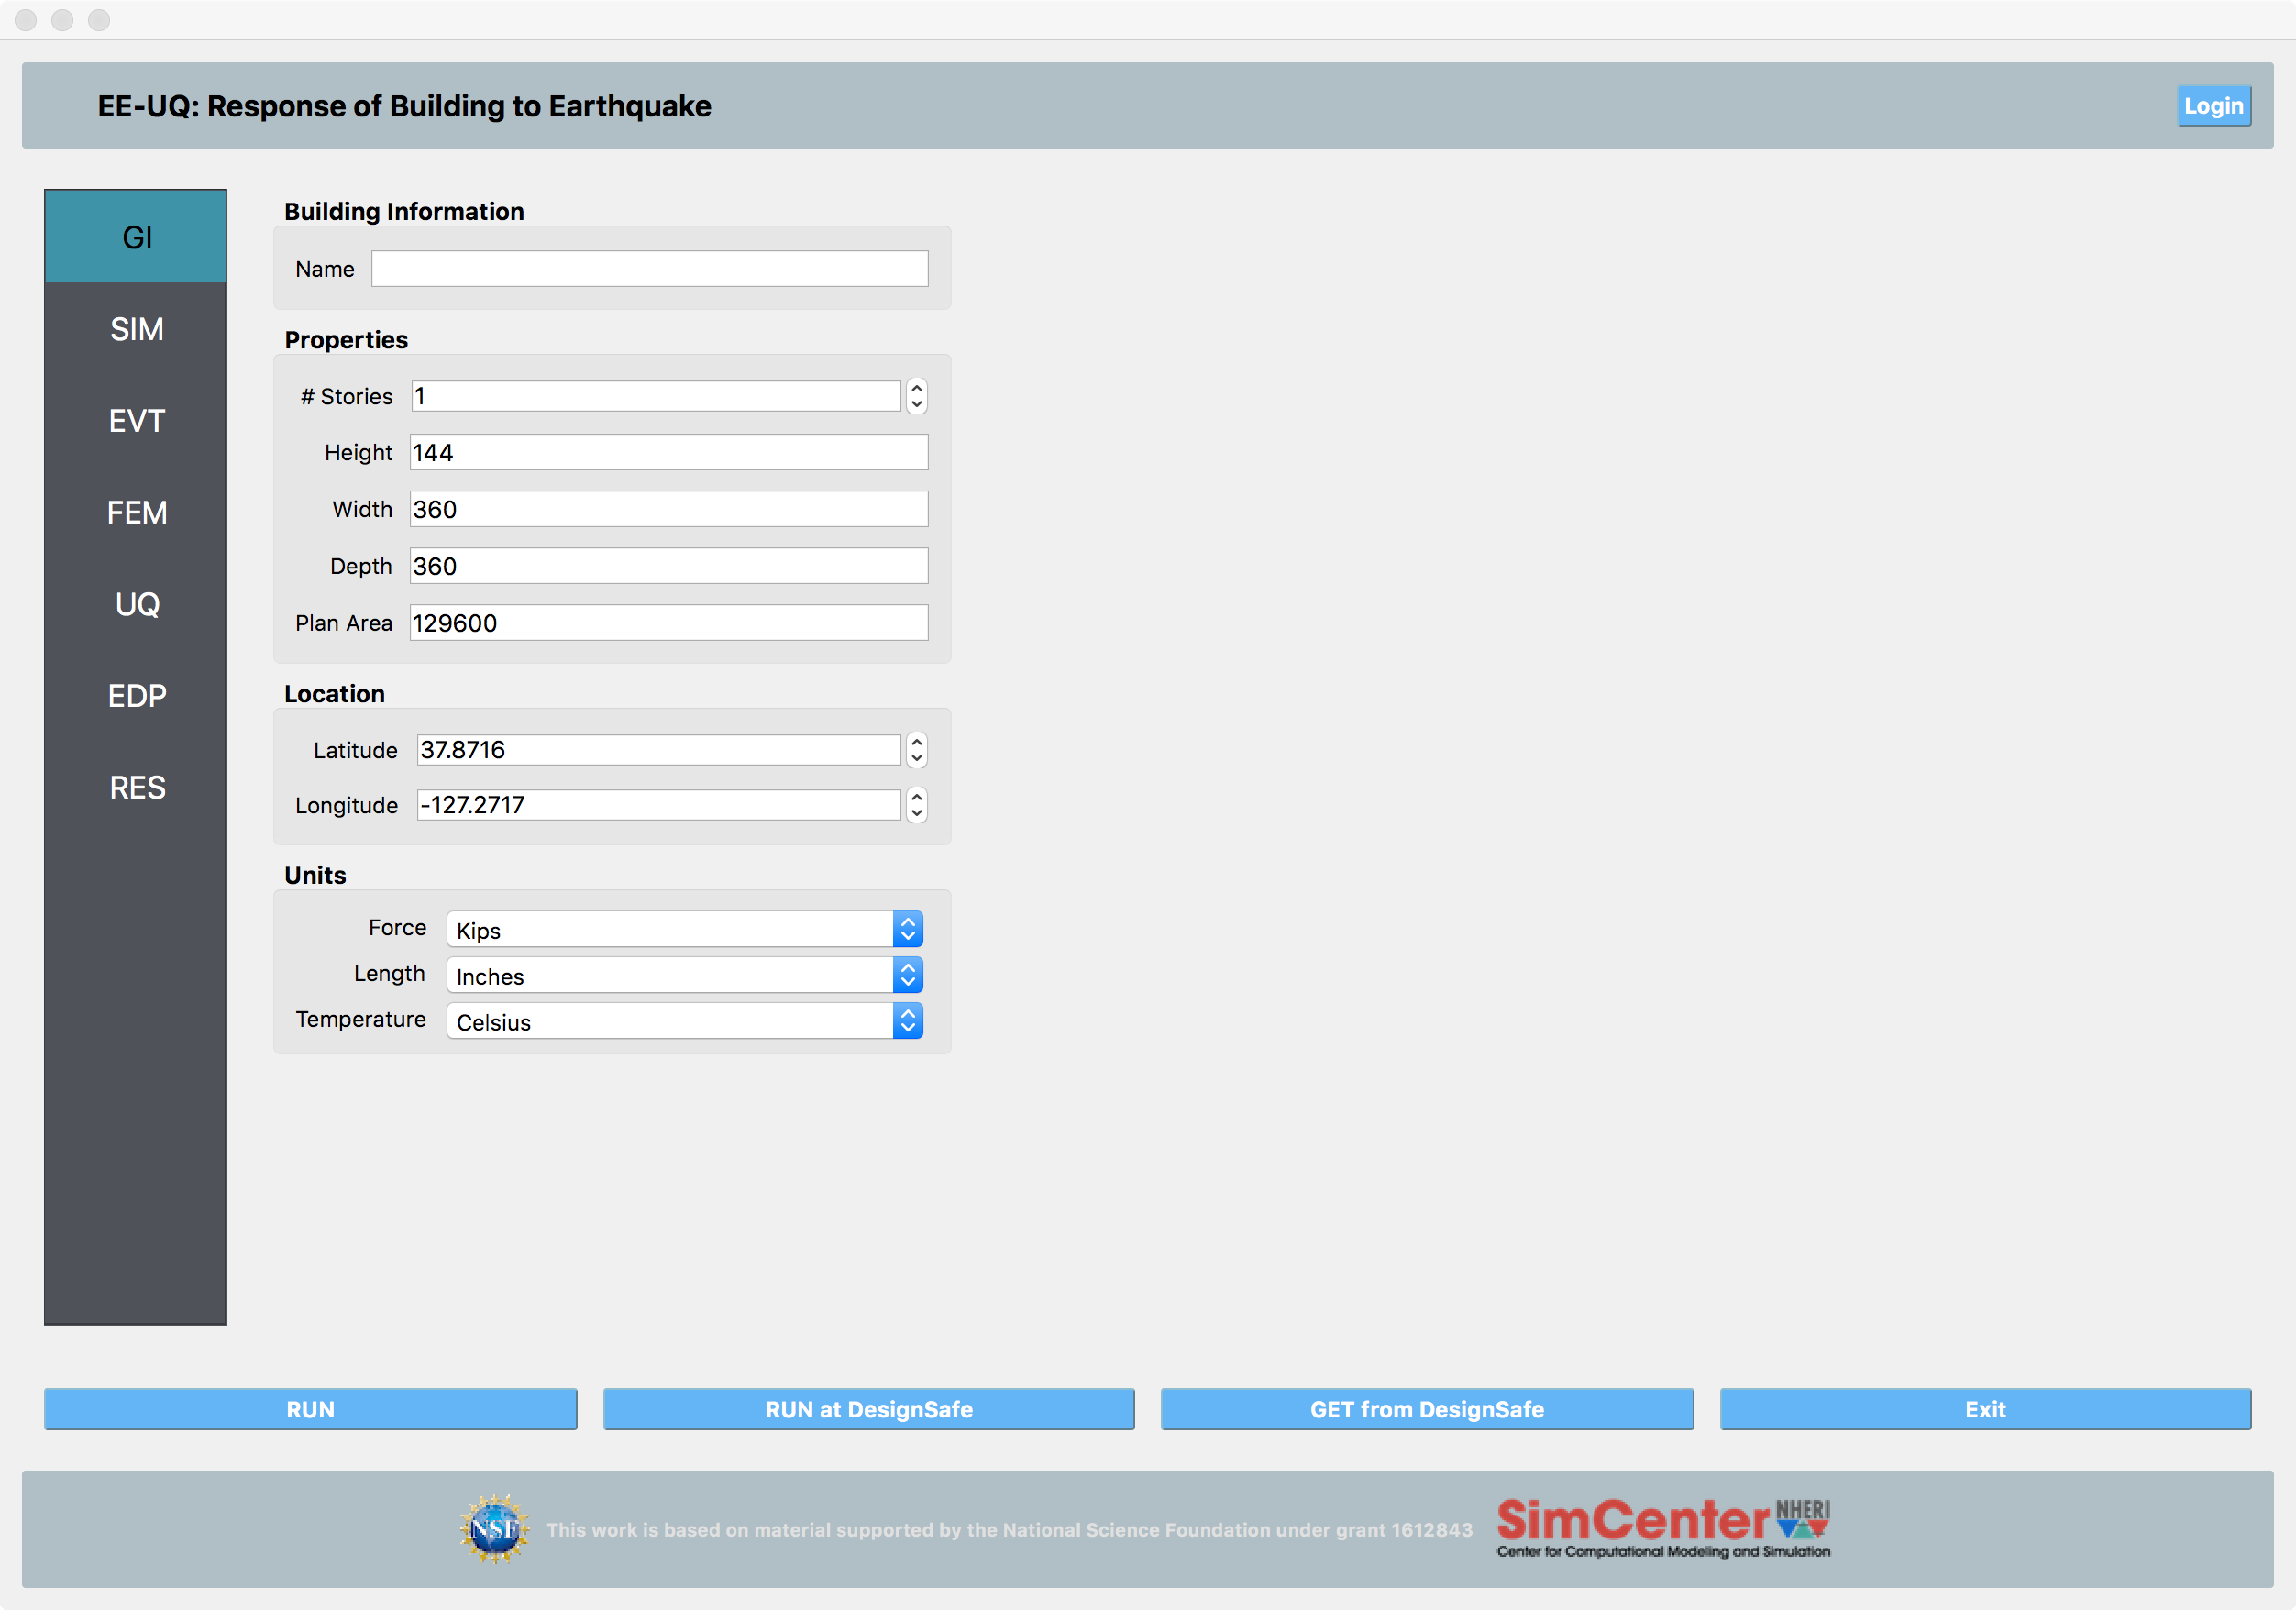
\includegraphics[width=0.95\textwidth]
    {installation/figures/EE-UQ.png} }
  \caption{EE-UQ Application on Startup}
  \label{fig:app_UI}
\end{figure}
}{}

\softwareSwitch{WE-UQ}{
\begin{figure}[!htbp]
  \centering {
    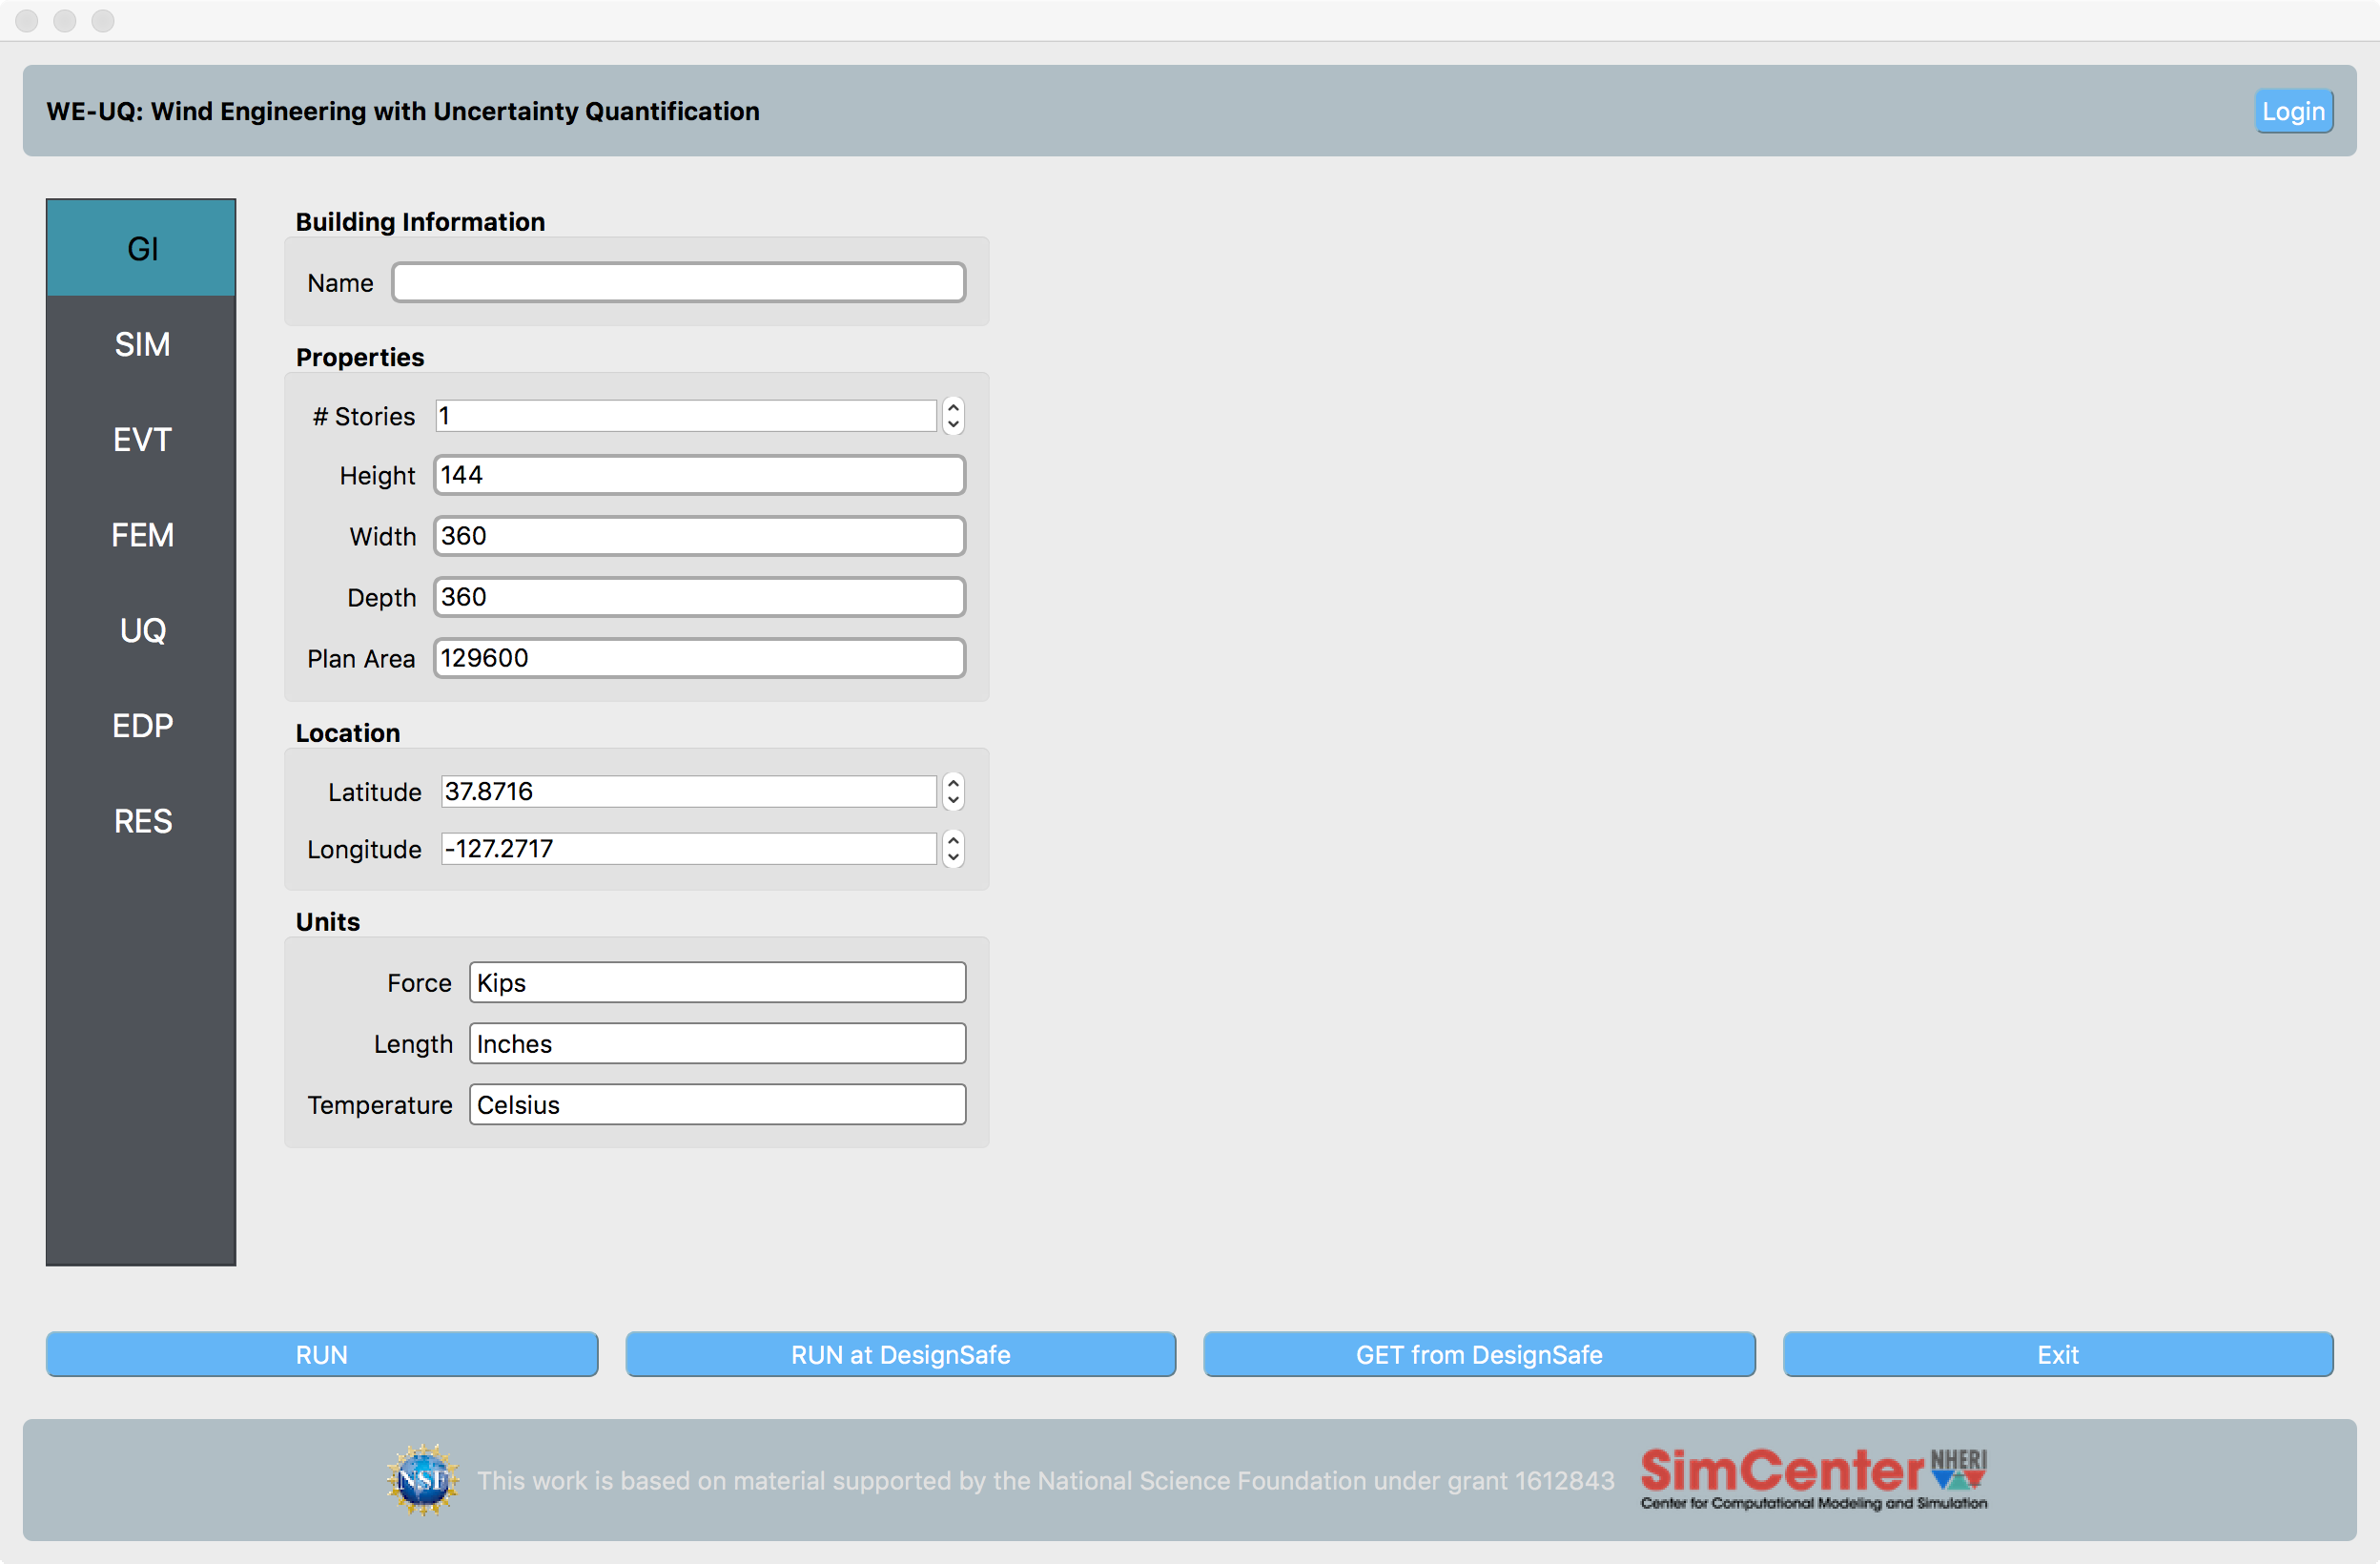
\includegraphics[width=0.95\textwidth]
    {installation/figures/WE-UQ.png} }
  \caption{WE-UQ Application on Startup}
  \label{fig:app_UI}
\end{figure}
}{}


\begin{enumerate}
\item The SimCenter is not recognized as either a Windows or an Apple vendor. Our applications are not recognized by the operating system as being signed. Consequently, you may receive a warning message when you start the \texttt{\getsoftwarename{}} application for the first time.
\item  On a Mac you will need to right click on the .dmg file to open it. The UI will not start correctly while in the DMG file, you need to open the .dmg file and then copy the \texttt{\getsoftwarename{}} application to your Documents or Desktop folder. You can then move the .dmg file to the trash or eject it after this has been done.
\item  The \texttt{\getsoftwarename{}} application requires additional software outlined in next subsections to work properly. Even of the software starts correctly, it will not run correctly until this software, outlined in the next section, is installed correctly.
\end{enumerate}


%===============================================================================
\section{Set up Python}
%===============================================================================

The SimCenter workflow applications are managed by Python
scripts. These are required to prepare the input data for running
analyses either remotely on DesignSafe or locally. As a consequence the user must have Python
installed on their machine and have the appropriate environment
variables set so that the UI can run these applications.

\subsection{Install Python}

SimCenter products require Python version 3.7 or above be installed on your machine as January 2020 marks the end of life for Python 2.7. 

\begin{enumerate}
\item Windows:

If you have not yet installed Python 3.7, we recommend installing from \href{https://www.python.org/downloads/windows}{Python.org}. We recommend installing using the \texttt{Windows x86-64 executable installer}.

Allow the installer to change your system environment variables so that the install directory is added to your PATH. Once installed you need to You need to install the following python packages: \texttt{numpy}, \texttt{scipy}, and \texttt{pandas} are installed. To install these packages open a \href{https://www.howtogeek.com/194041/how-to-open-the-command-prompt-as-administrator-in-windows-8.1/}{terminal window as an Admin user} and in that window type the following instructions:

To install these packages, start a terminal window and type:

\begin{verbatim}
pip install numpy
pip install scipy
pip install pandas
\end{verbatim}

\item Mac

The Mac comes with Python pre-installed, which is currently the somewhat 
dated version 2.7. To install Python 3.7 we recommend installing from 
\href{https://www.python.org/downloads/}{Python.org}. We recommend installing using the 
\texttt {macOS 64-bit installer} given for latest stable release. The installer will place a python3 executable in your /usr/local/bin directory, whose location should be on your system PATH.

You need to install the following python packages: \texttt{numpy}, \texttt{scipy}, and \texttt{pandas} are installed. 
To install these packages, start a terminal window and type:

\begin{verbatim}
pip3 install numpy
pip3 install scipy
pip3 install pandas
\end{verbatim}

Notes: 
\begin{enumerate}
\item To start a terminal window you can use the spotlight app (magnifying top right of desktop). Start the spotlight app and type in terminal. The terminal application should appear as the top hit. Click on it to start it.
\item In tool preferences make sure that python3 appears as the python executable. If you used older versions of SImCEnter tools this was the default.
\end{enumerate}
\end{enumerate} 

\subsection{Test Python}
%===============================================================================

Test if the python environment is set up properly by
executing \texttt{python} in a terminal window. After Python starts,
test if the packages are installed by executing \texttt{import
numpy}, \texttt{import scipy}, and \texttt{import pandas}. You will
receive an error message if a pacakage is missing. If no error
appears, the terminal should look similar
to \Cref{fig:python_test}. Exit Python by executing
the \texttt{exit()} command.

\begin{figure}[!htbp]
  \centering {
    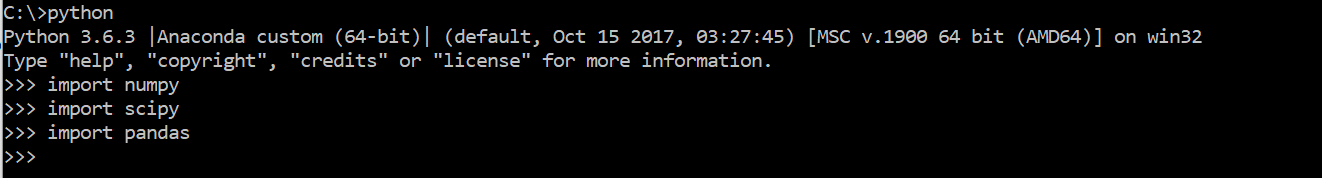
\includegraphics[width=0.8\textwidth]
    {installation/figures/python_test.png} }
  \caption{Testing the Python environment.}
  \label{fig:python_test}
\end{figure}

%===============================================================================
\section{Set up for Running Workflows Locally}\label{setup}
%===============================================================================

To run the workflows locally, the backend python application needs
publicly available software to also be installed on your
machine. These software applications need to be installed and
configured on your operating system. If you do not plan to run the
workflows locally, you will not need these applications.


\subsection{Install \texttt{OpenSees}}
%===============================================================================

\href{http://opensees.berkeley.edu}{\texttt{OpenSees}} is an open-source finite element application publicly available for download from its \href{http://opensees.berkeley.edu/OpenSees/user/download.php}{download page}. \texttt{OpenSees} installation requires the user install both \texttt{OpenSees} and \texttt{Tcl}.  If you have never downloaded \texttt{OpenSees} before, you will need to register your e-mail to gain access. After registration, you can proceed to the download page by entering your email address and clicking the Submit button. The Windows and Mac downloads are in different locations on the download page, with the appropriate Tcl installer beside the \texttt{OpenSees} link; see \Cref{fig:openseesDownload}

\begin{figure}[!htbp]
  \centering {
    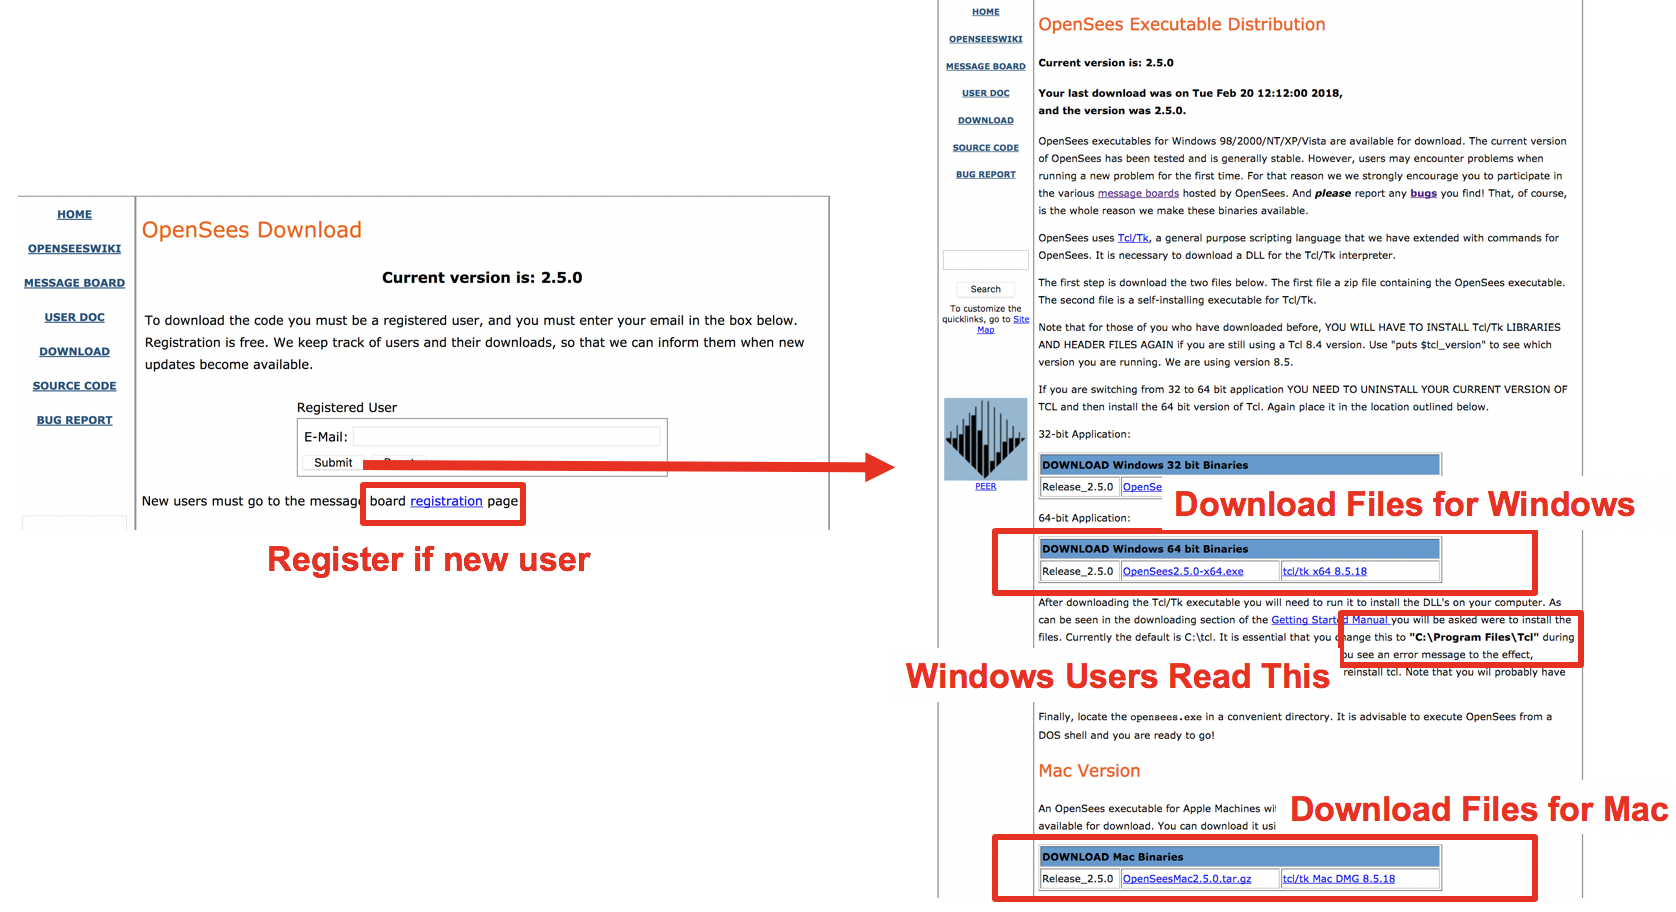
\includegraphics[width=\textwidth]
    {installation/figures/openseesDownload.png} }
  \caption{Downloading OpenSees}
  \label{fig:openseesDownload}
\end{figure}

Follow the instructions on the download page to install \texttt{Tcl}
(\Cref{fig:openseesDownload}). On Windows, you must select the Custom option for installton and you must specify
the installtion directory as \texttt{C:\textbackslash Program Files\textbackslash Tcl}, 
which is not the default. \\

After \texttt{Tcl} is installed, we recommend you put \texttt{OpenSees} in
the \texttt{C:/SimCenter/OpenSees} folder on Windows and in
a \texttt{/usr/local/OpenSees} directory on the Mac (If you use finder
on Mac to do navigation, use command-shift-G in Finder and specify
/usr/local as the folder to go to. Create a new folder \texttt{OpenSees}
and copy the \texttt{OpenSees} application to this folder).\\


Now you need to add the \texttt{OpenSees} folder to the
system \texttt{PATH} environment variable to allow the SimCenter
workflow applications to find the \texttt{OpenSees} executable on your
computer. The steps to do this depend on your operating system:

\begin{enumerate}
\item Windows: To add a folder to the \texttt{PATH} on Windows (\Cref{fig:add_env_path}):

\begin{figure}[!htbp]
  \centering {
    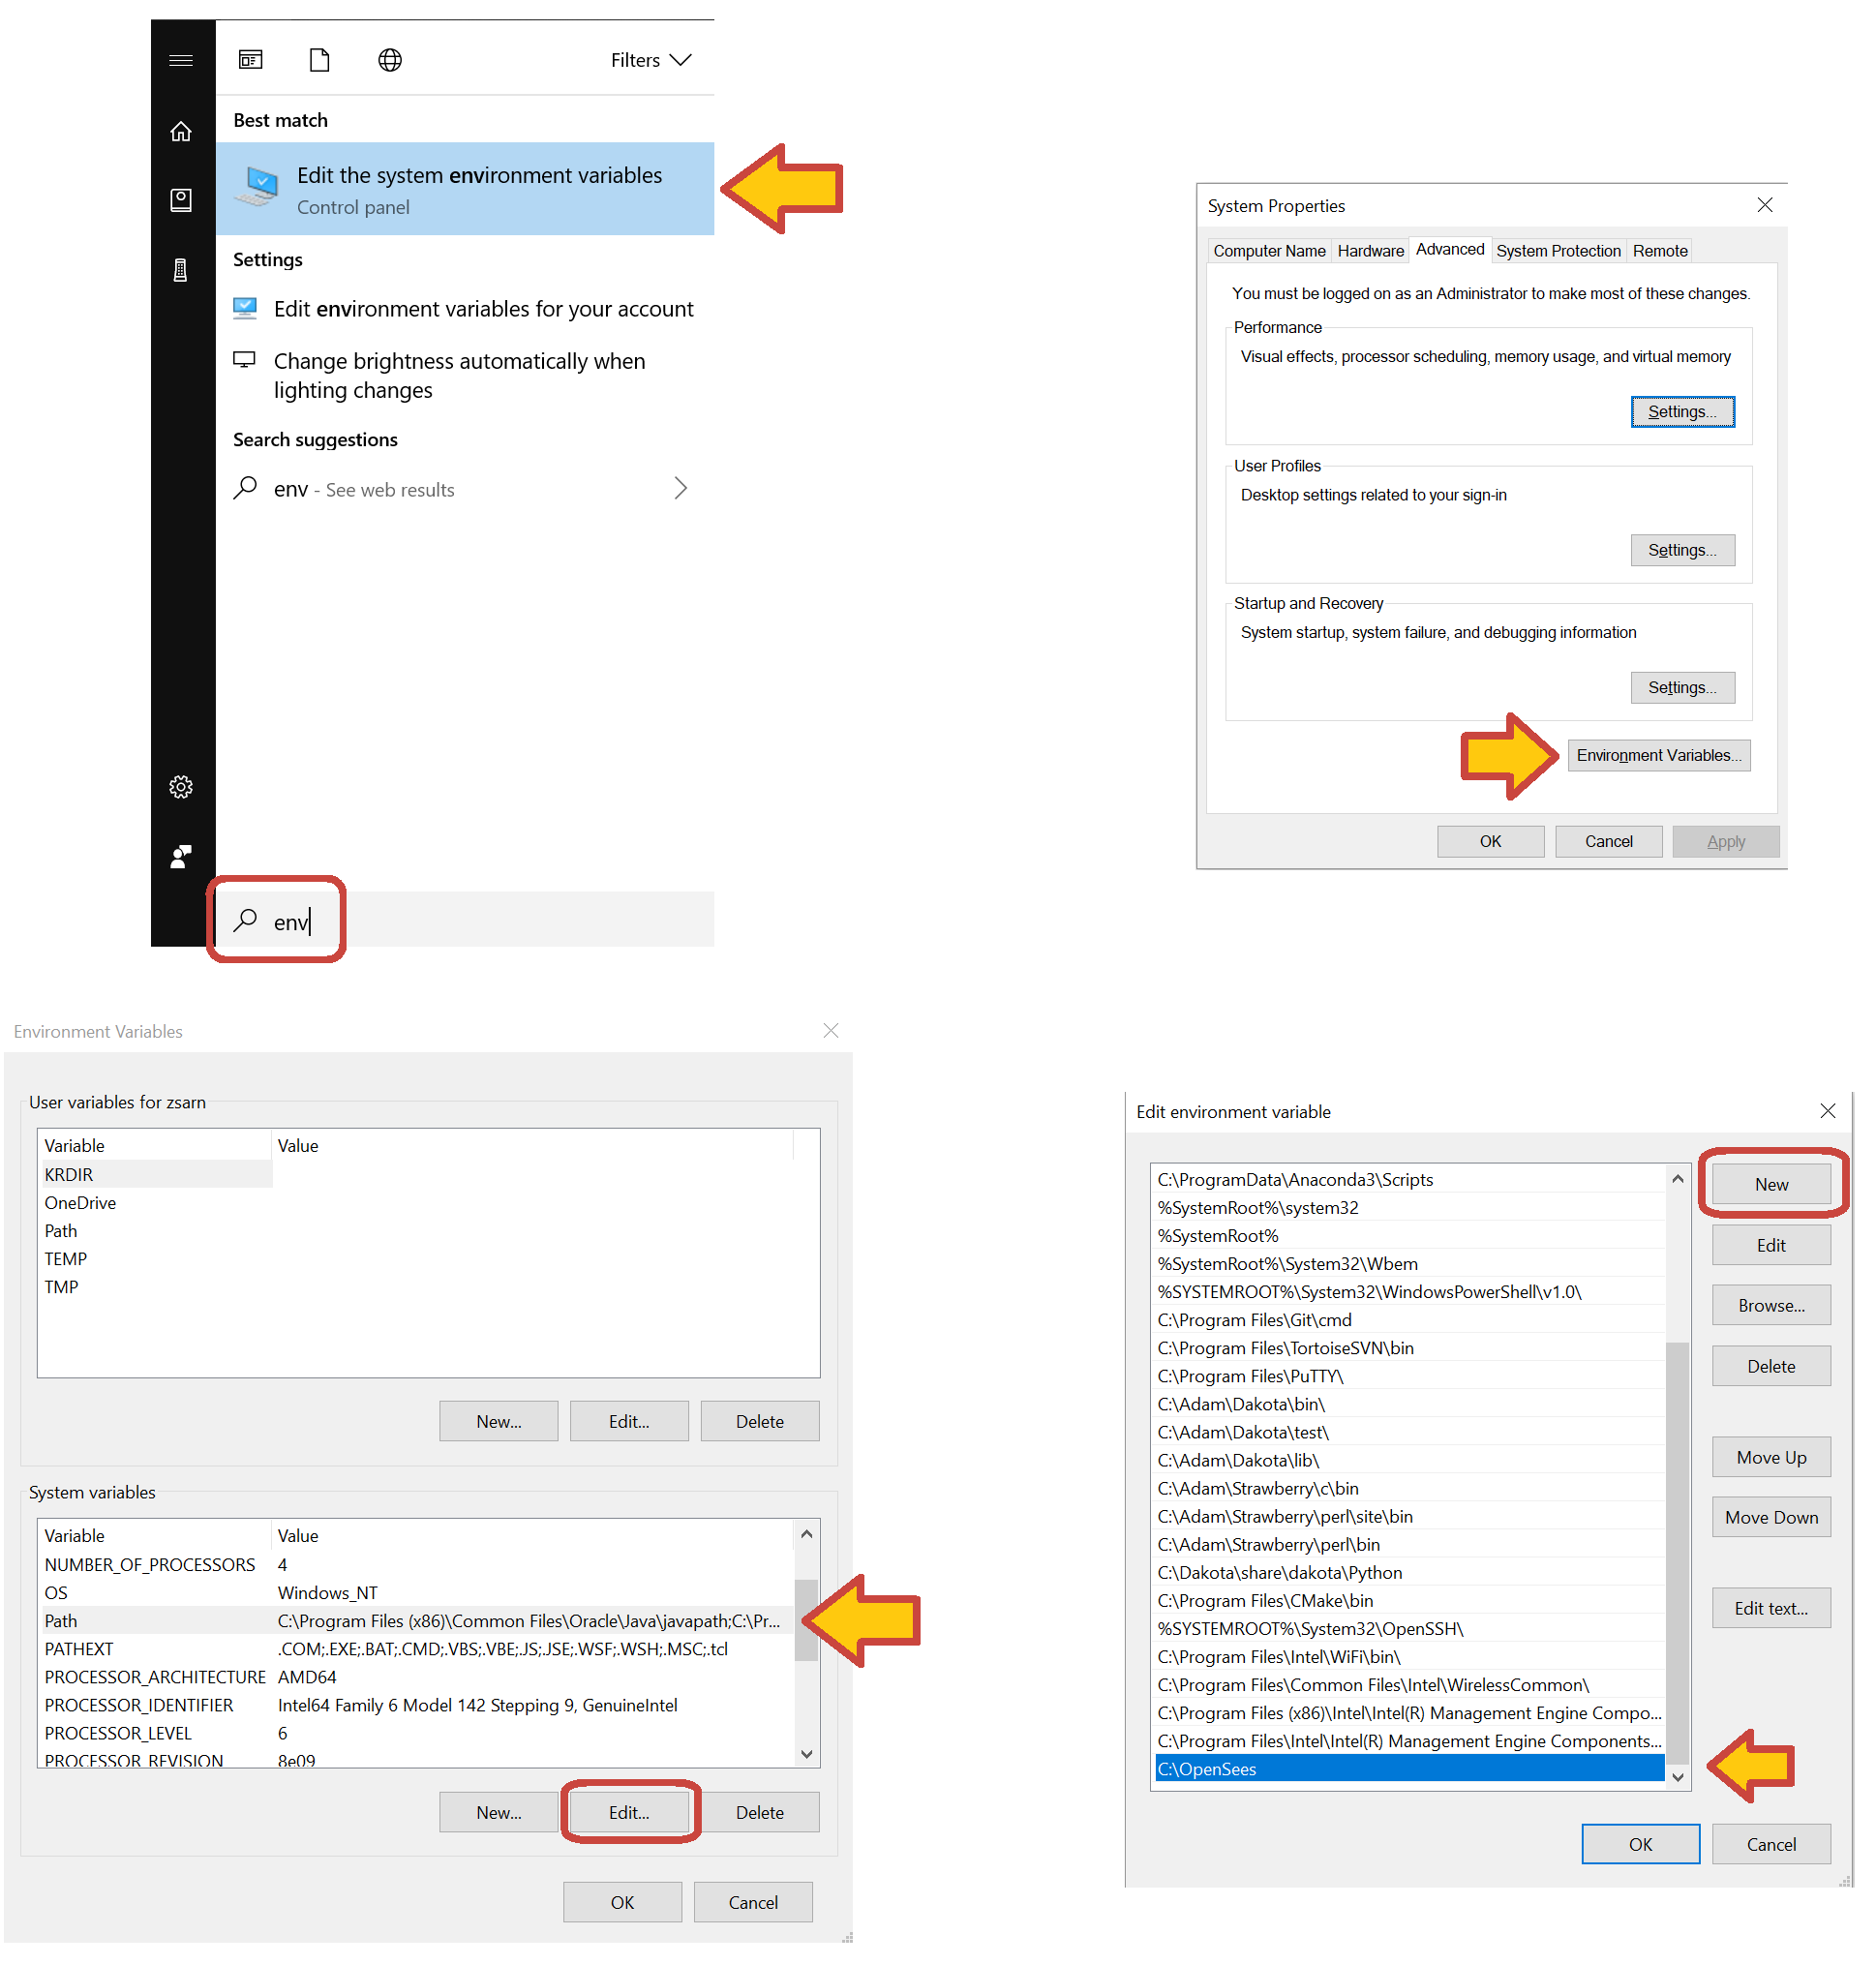
\includegraphics[width=0.8\textwidth]
    {installation/figures/add_env_path.png} }
  \caption{Adding OpenSees to the PATH environment variable on Windows}
  \label{fig:add_env_path}
\end{figure}


\begin{enumerate}
    \item open \emph{Start}, type \emph{env}, and choose \emph{Edit the system environment variables};
    \item click on the \emph{Environment variables...} button in the dialog window;
    \item find the \texttt{Path} under \emph{System Variables} in the \emph{Variable} column;
    \item click \emph{New} and type in the path to your \texttt{OpenSees.exe} (this will be \texttt{C:\textbackslash SimCenter\textbackslash OpenSees} if you put the executable at the recommended location - pay attention to using backslashes here!);
    \item click \emph{OK} in every dialog to close them and save your changes.
\end{enumerate}

\item MacOS: To add the /usr/local/OpenSees folder to the \texttt{PATH} variable:

\begin{enumerate}
    \item open a Terminal;
    \item execute (type the following in the terminal window and hit the return key) the following: \begin{verbatim}nano ${HOME}/.bash_profile\end{verbatim}
    \item if the file contains nothing, add the first 3 lines shown in \Cref{fig:add_env_path_Mac} to the file. This is done in
case an existing .bashrc file exists for your system. Adding these 3 lines will test for the existance of this file, and source in any existing commands if the file does exist.
    \item on a new line add the \texttt{OpenSees} executable to the PATH variable, by typing the following: \begin{verbatim}export PATH=/usr/local/OpenSees:${PATH}\end{verbatim}
    \item quit by hitting \texttt{Ctrl+X} and then \texttt{Y} when asked if you want to save modifications.
    \item test it is entered correctl, the following command now entered in the terminal window should result in no errors: \begin{verbatim}source ${HOME}/.bash_profile\end{verbatim}. 
\end{enumerate}

\begin{figure}[!htbp]
  \centering {
     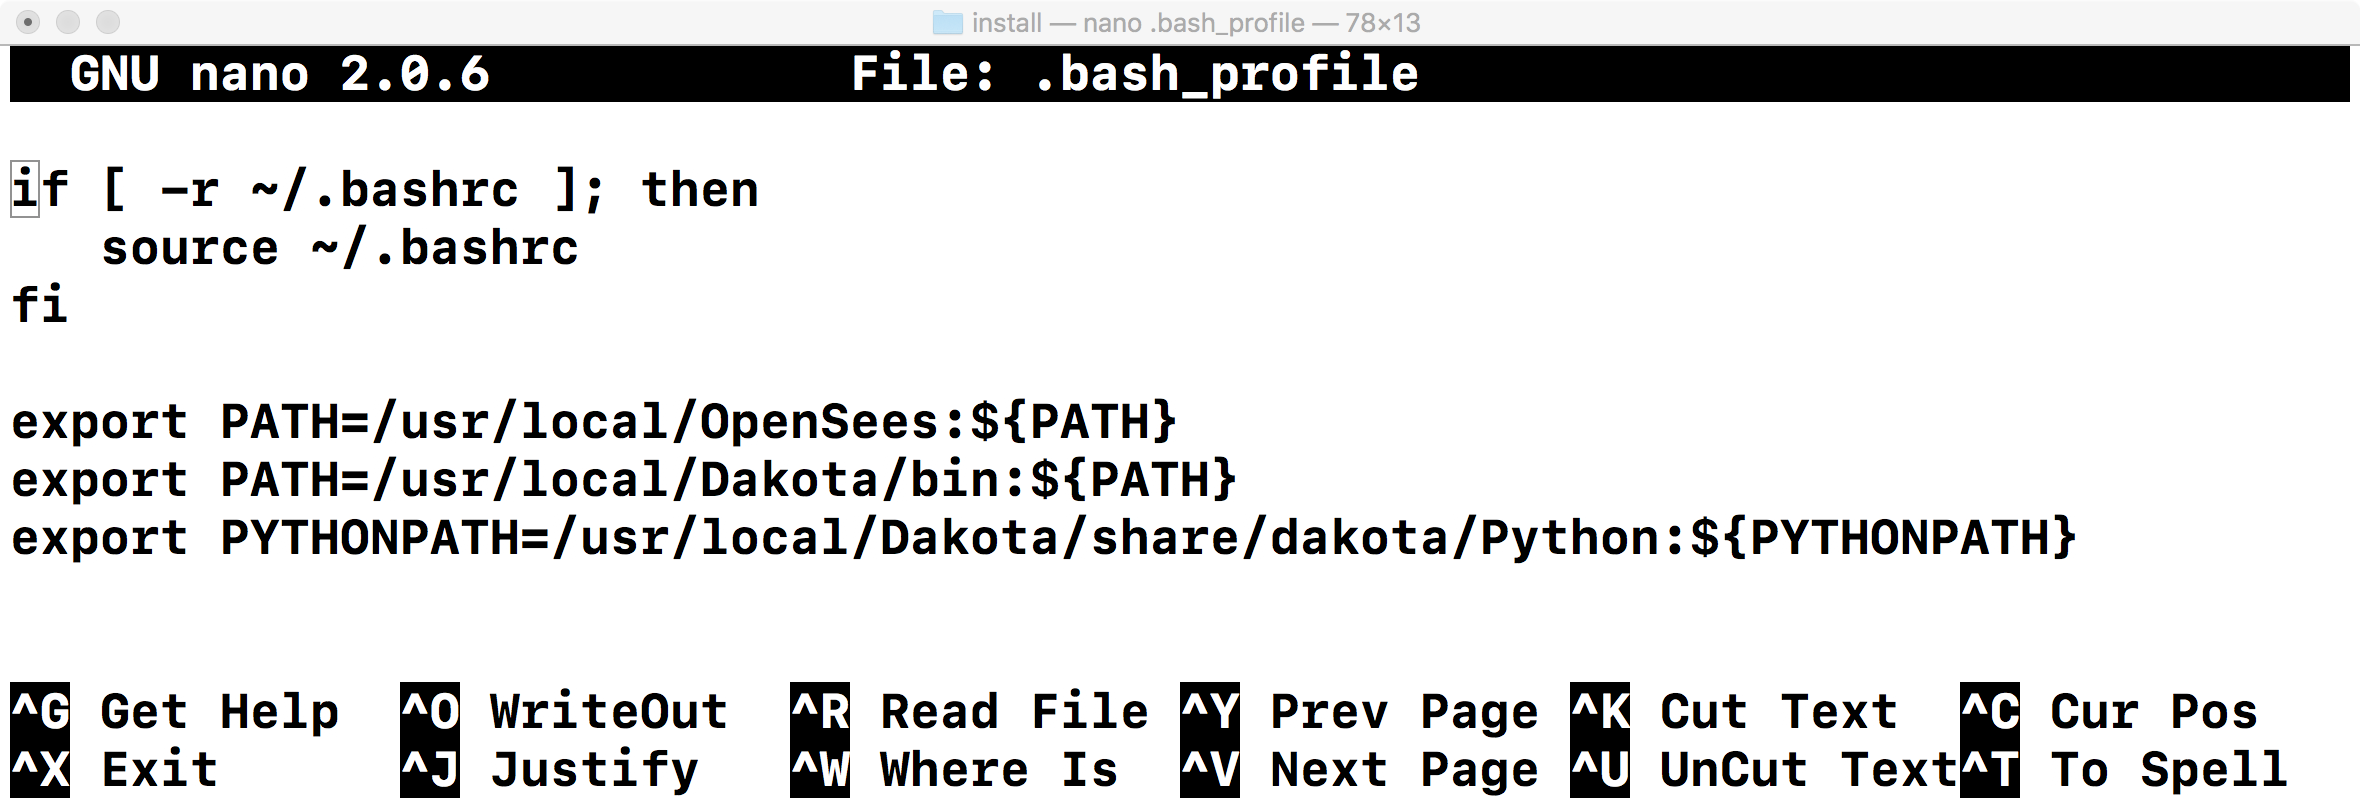
\includegraphics[width=0.8\textwidth]
    {installation/figures/add_env_path_Mac.png} }
  \caption{Adding OpenSees to the PATH environment variable on Mac.}
  \label{fig:add_env_path_Mac}
\end{figure}


\end{enumerate}


\subsection{Install \texttt{FEAPpv}}
%===============================================================================

\href{http://projects.ce.berkeley.edu/feap/feappv/}{\texttt{FEAPpv}} is a general purpose finite element analysis program which is designed for research and educational use. The program is the companion to the books: \texttt{The Finite Element Method, 7th edition, Volumes 1 and 2 (but not Vol 3)}, authored by O.C. Zienkiewicz and R.L. Taylor and published by Elsevier, Oxford, 2013.  Pre-built executables are available for download from the main \href{http://projects.ce.berkeley.edu/feap/feappv/}{web page}.


We recommend you put \texttt{FEAPpv} in
the \texttt{C:/SimCenter/FEAPpv} folder on Windows and in
a \texttt{/usr/local/FEAPpv} directory on the Mac (If you use finder
on Mac to do navigation, use command-shift-G in Finder and specify
/usr/local as the folder to go to. Create a new folder \texttt{FEAPpv}
and copy the \texttt{FEAPpv} application to this folder).\\


Now you need to add the \texttt{FEAPpv} folder to the
system \texttt{PATH} environment variable to allow the SimCenter
workflow applications to find the \texttt{FEAPpv} executable on your
computer. The steps to do this are similar to those just described for installing OpenSees.


\subsection{Install \texttt{Dakota}}
%===============================================================================

\href{http://dakota.sandia.gov}{\texttt{Dakota}}, an open-source  optimization and UQ application from Sandia National Labs, is publicly available for download at its \href{http://dakota.sandia.gov/download.html}{download page}. Select your operating system from the list and set the other options as shown in  \Cref{fig:dakota_installation}. Download the release in a \texttt{ZIP} file for Windows and \texttt{TAR.GZ} file for Mac. We recommend you to extract the archive to a \texttt{C:/SimCenter/Dakota} folder on Windows, and to a \texttt{/usr/local/Dakota} folder on a Mac.

\begin{figure}[!htbp]
  \centering {
    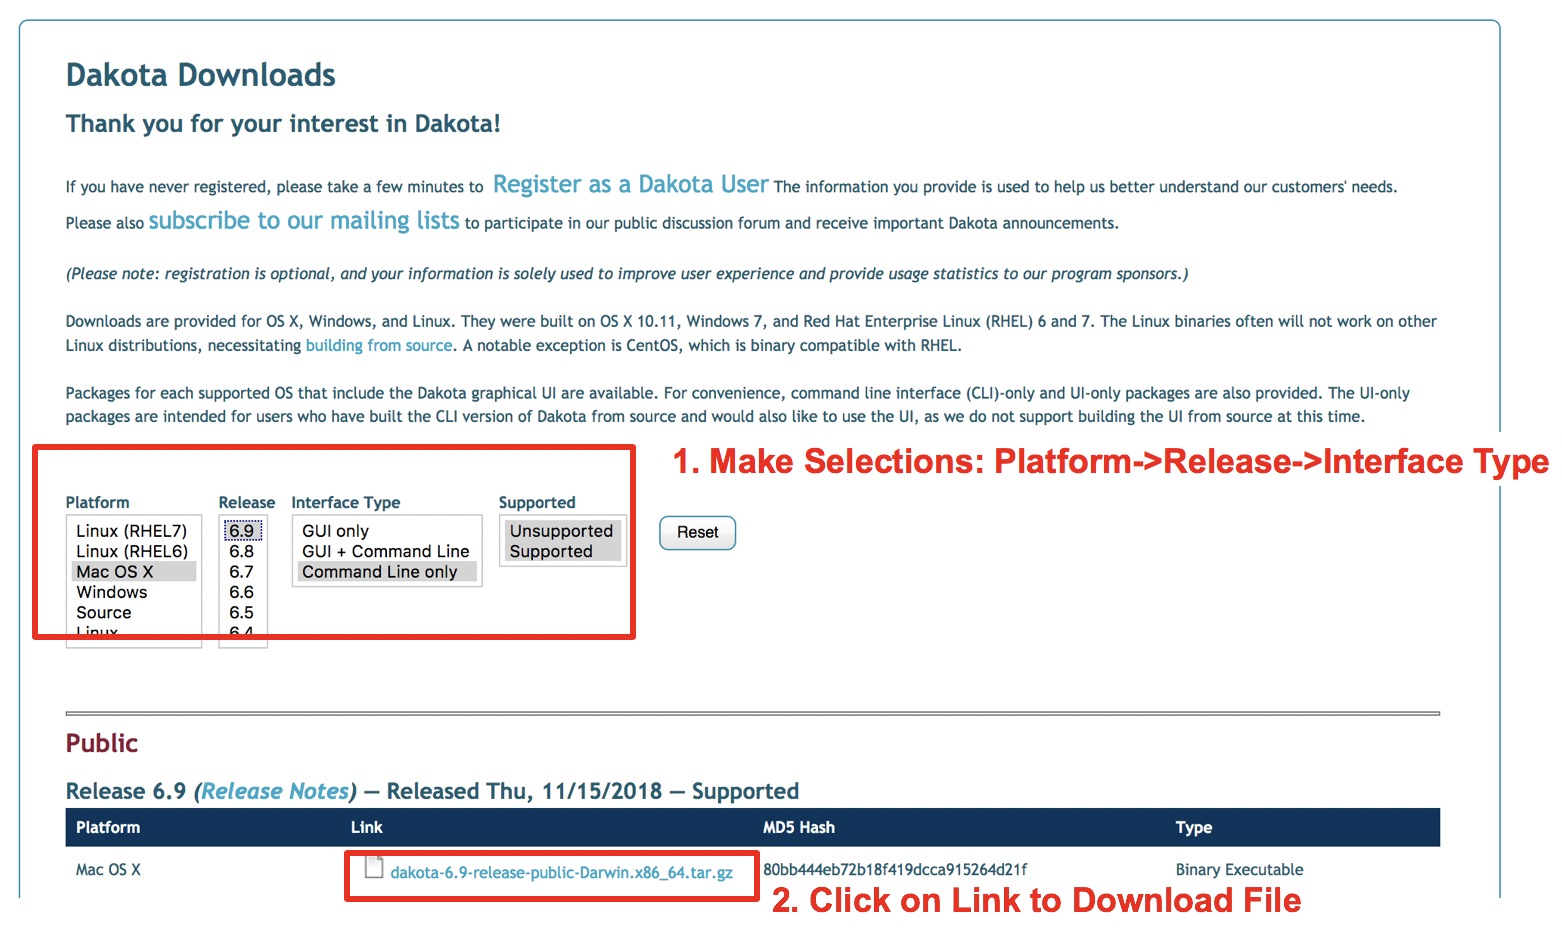
\includegraphics[width=\textwidth]
    {installation/figures/dakota_installation.png} }
  \caption{Downloading Dakota Software}
  \label{fig:dakota_installation}
\end{figure}


Following the instructions provided for installing \texttt{OpenSees}, you need to add \textbf{two} \texttt{Dakota} folders to the system \texttt{PATH} environment variable to allow the SimCenter workflow applications to find the \texttt{Dakota} tools on your computer. 
the procedure described above for \texttt{OpenSees} to add the following
folders to your \texttt{PATH}:

\begin{enumerate}
\item{Windows}

Add the following 2 folders to your windows PATH variable:
\begin{itemize}
    \item \texttt{C:\textbackslash SimCenter\textbackslash Dakota\textbackslash bin}
    \item \texttt{C:\textbackslash SimCenter\textbackslash Dakota\textbackslash share\textbackslash dakota\textbackslash Python}
\end{itemize}

Now you need to create a new variable, \texttt{PYTHONPATH}, and point it to the following folder.


\begin{itemize}
    \item \texttt{C:\textbackslash SimCenter\textbackslash Dakota\textbackslash share\textbackslash dakota\textbackslash Python}
\end{itemize}

\item{MacOS}
On the Mac you also need to add 2 lines, previously shown in \Cref{fig:add_env_path_Mac},
 to the .bash\_profile file. One line adds the Dakota executable to the PATH variablem and 
the other creates a new variable PYTHONPATH and points it to a folder in the  Dakota 
installation directory. 

\begin{itemize}
    \item \texttt{export PATH=/usr/local/Dakota/bin:\${PATH}}
    \item \texttt{export PYTHONPATH=/usr/local/Dakota/share/dakota/Python}
\end{itemize}
\end{enumerate}

NOTE: Apple, in the latest release of their operating system, MacOS 10.16 Catalina, has changed the default working of Gatekeeper.
Gatekeeper, first introduced in OS X Mountain Lion, is a Mac security feature that helps protect your Mac from Malware and other malicious software. Gatekeeper checks to make sure the application is safe to run by checking it against the list of apps that Apple has vetted and approved for the Apple Mac Store and/or approved by Apple even if not offered through the app store. In previous versions of MacOS, Gatekeeper had three security level options: App Store, App Store and Identified Developers, and Anywhere. Anywhere has been removed and this will cause problems with Dakota. As a consequence, it is necessary to follow the following when you update the MacOS or install Dakota for the first time on machine with an updated MacOS. From the terminal app, with the above .bash\_profile settings set, you need to type the following in the terminal window:

\begin{verbatim}
sudo spctl --master-disable
dakota
sudo spctl --master-enable
\end{verbatim}

This will temporarily disable gatekeeper (basically setting Gatekeeper options to Anywhere), allow the Dakota application and it's .dylib files to be registered as safe, and then turn Gatekeeper options back to default.



\subsection{Test the Install of the Local Applications}
%===============================================================================

Before running the \texttt{\getsoftwarename{}} application, perform the following tests to
make sure that the local SimCenter working environment is set up
appropriately:

\begin{itemize}
    \item Start a Terminal on Mac or a Command Prompt on Windows.
    \item On Mac, execute \texttt{cd /usr/Documents} to change the active directory to \texttt{/usr/Documents}. On Windows, execute \texttt{cd C:/} to change the active directory to \texttt{C:/}.
    \item Test if \texttt{OpenSees} works correctly by executing the \texttt{OpenSees} command. The command should start \texttt{OpenSees} (\Cref{fig:opensees_test}). Close \texttt{OpenSees} with the \texttt{exit} command.
    \item Test if \texttt{Dakota} works correctly by executing the \texttt{dakota} command. The command should start \texttt{Dakota} and you should see a message about a missing argument (\Cref{fig:dakota_test}).
    \item Test if the python package in \texttt{Dakota} works correctly by starting Python with the \texttt{python} command and then executing the \texttt{import dakota} command. This should import the dakota package. If you do not see errors, then the package is successfully imported (\Cref{fig:dakota_py_test}). Exit Python with the \texttt{exit()} command.
    \item If all the above tests ran without errors, your environment is set up appropriately.
\end{itemize}

\begin{figure}[!htbp]
  \centering {
    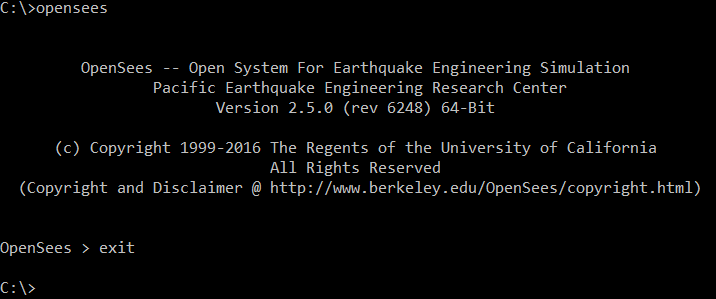
\includegraphics[width=0.8\textwidth]
    {installation/figures/opensees_test.png} }
  \caption{Testing OpenSees.}
  \label{fig:opensees_test}
\end{figure}

\begin{figure}[!htbp]
  \centering {
    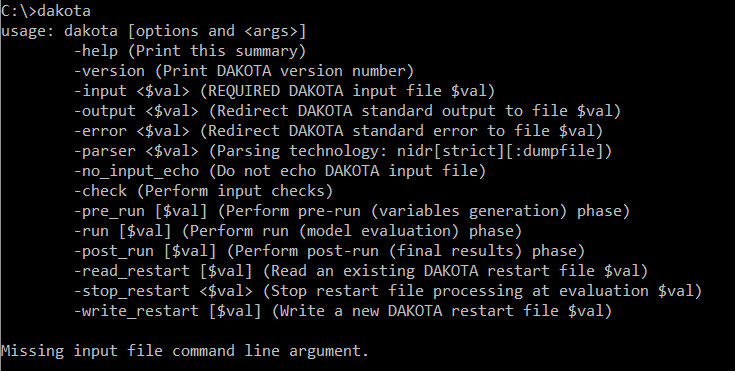
\includegraphics[width=0.8\textwidth]
    {installation/figures/dakota_test.png} }
  \caption{Testing Dakota.}
  \label{fig:dakota_test}
\end{figure}

\begin{figure}[!htbp]
  \centering {
    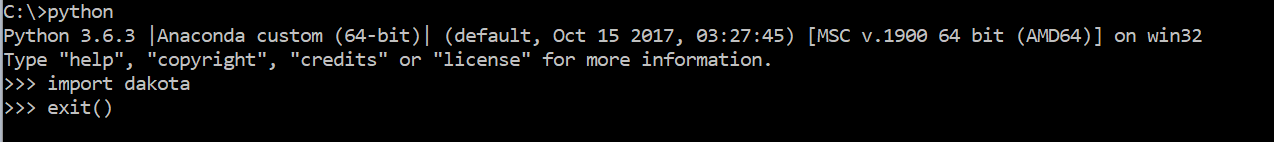
\includegraphics[width=0.8\textwidth]
    {installation/figures/dakota_py_test.png} }
  \caption{Testing the dakota Python package.}
  \label{fig:dakota_py_test}
\end{figure}

